\chapter{docker 이미지 만들기}
우리는 이제 docker를 이용하여 서버를 설치할 수 있다. 몇번의 명령어를 실행하면 이미 만들어져 있는 서버를 순식간에 만들어낼 수 있다니 놀랍지 않나요? 이번 장에서는 앞에서 설치한 ststic-site를 수정하여 나만의 static site로 만드는 방법을 학습한다. 이 때 중요한 명령어는 commit이다. 

\section{commit하기}
지금 여러분의 컴퓨터에 설치되어 있는 이미지가 어떤 것들이 있는지 살펴보자. 
아래 명령어를 실행하면 현재 다운로드 되어 있는 이미지를 볼 수 있다. 이 이미지를 컨테이너에 넣은 다음 실행해야 서버가 동작한다. `docker images` 를 실행하면 의 이미지가 나열된 결과를 볼수 있고, 지난 시간에 사용하였던 static-site가 보인다. 이 도커 이미지를 컨테이너에 넣고 실행하자. 아래와 같이 실행하면 된다. 이 도커 이미지를 실행시키고 myserver라고 이름 붙인다. 컨테이너를 실행 후 firefox를 열어 http://localhost:8080/ 에 접속하면 웹사이트를 볼 수 있다. 

\begin{tikzpicture}[node distance=2.5cm, auto]

    % Nodes
    \node (search) [process] {Search Docker Image};
    \node (download) [process, below of=search, xshift=3cm] {Download Docker Image};
    \node (create) [process, below of=download] {Create Container};
    \node (start) [process, below of=create] {Start Container};
    \node (stop) [process, below of=start] {Stop Container};
    \node (restart) [process, left of=stop, xshift=-3cm] {Restart Container};
    \node (remove) [process, above of=restart] {Remove Container};
    \node (rmi) [process, above of=remove] {Remove Docker Image};

    % Arrows
    \draw [arrow] (search) -- (download);
    \draw [arrow] (download) -- (create);
    \draw [arrow] (create) -- (start);
    \draw [arrow] (start) -- (stop);
    \draw [arrow] (stop) -- (restart);
    \draw [arrow] (restart) -- (remove);
    \draw [arrow] (remove) -- (rmi);
    \draw [arrow] (rmi) -- (search);

\end{tikzpicture}

\begin{lstlisting}
$ sudo docker images 
REPOSITORY                TAG       IMAGE ID       CREATED         SIZE
mynginx                   latest    3ee48dfc2712   14 hours ago    249MB
nginx                     latest    5ef79149e0ec   12 days ago     188MB
busybox                   latest    65ad0d468eb1   15 months ago   4.26MB
hello-world               latest    d2c94e258dcb   16 months ago   13.3kB
prakhar1989/static-site   latest    f01030e1dcf3   8 years ago     134MB

$ sudo docker run -it -d -p 8080:80 --name myserver prakhar1989/static-site
ec12360056844129f863e79a30869887eee0c4ee87a9e3ea69b2a9aa309af5b0
\end{lstlisting}

이제 이 웹사이트를 수정하려면 컨테이너 안으로 들어가야 한다. 컨테이너에 접속하여 작업을 하기 위해서는 다음과 같은 명령어가 필요하다. 이제 컨테이너 안에서 작업할 수 있다. 작업을 위해 /usr/share/nginx/html/ 이동하고, ls 명령어를 이용하여 파일을 확인한다. 이제 index.html을 수정하여 나만의 홈페이지를 만든다. 
\begin{lstlisting}[language=bash]
# docker exec -it [container name] /bin/bash
$ sudo docker exec -it myserver /bin/bash
root@ec1236005684:/# 
root@ec1236005684:/# cd /usr/share/nginx/html/
root@ec1236005684:/usr/share/nginx/html# ls
50x.html  css  images  index.html
root@ec1236005684:/usr/share/nginx/html# 
\end{lstlisting}

index.html 파일을 수정하기 위해서 vi 에이터를 사용해 본다. 자신이 익숙한 에디터를 사용해도 된다. vi 에디터가 없다면 cat명령어 사용법을 공부한 후 시도 해본다. 

\begin{figure}[htp]
    \centering
    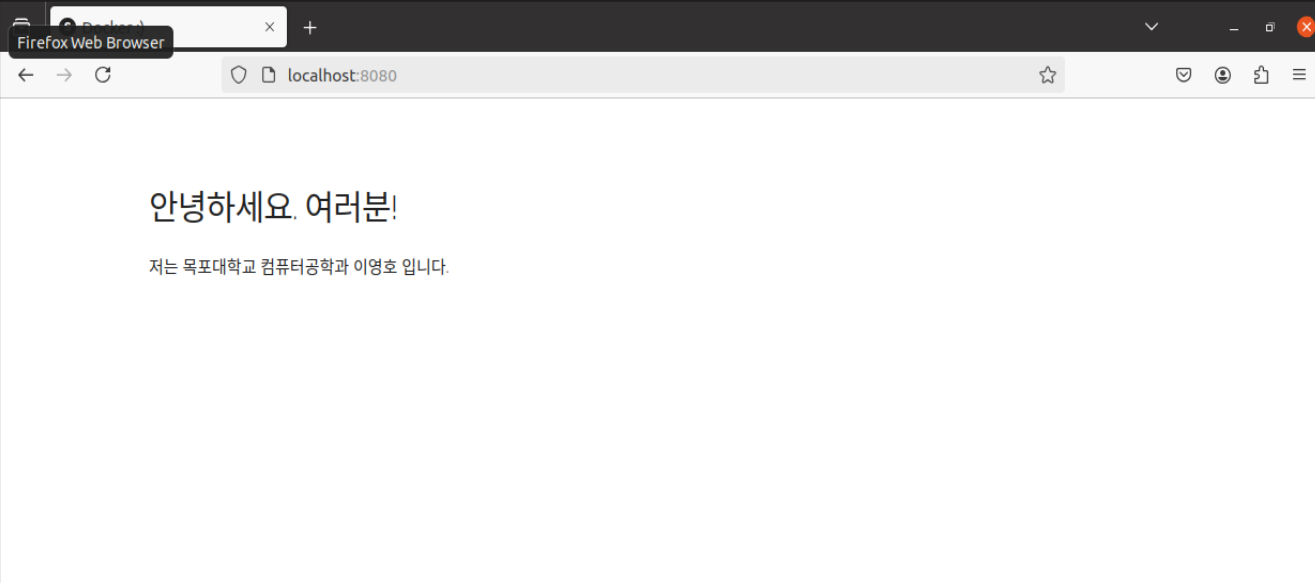
\includegraphics[width=\textwidth]{images/chaptert5images/image.png}
\end{figure}

이제 여러분은 도커 이미지를 받아 새로운 서버를 만들 수 있게 되었다. 하지만 컨테이너는 읽기만 가능하고 쓰기는 불가능하다. 즉, 실행종료 후에 다시 실행하면 여러분의 작업 내용은 삭제된다. 따라서 새로운 도커 이미지, 즉 여러분 만의 도커 이미지를 만들 수 있어야 한다. 

\begin{lstlisting}[language=bash]
root@ec1236005684:/usr/share/nginx/html# exit
    exit
$ sudo docker stop myserver 
    myserver
$ sudo docker commit myserver mynewserver
sha256:3372a92d9e3f83605e5149ccf794a4b85121f023738f8e76a7d74896e1c199bc
$ sudo docker images
    REPOSITORY                TAG       IMAGE ID       CREATED         SIZE
    mynewserver               latest    3372a92d9e3f   7 seconds ago   134MB
    mynginx                   latest    3ee48dfc2712   14 hours ago    249MB
    nginx                     latest    5ef79149e0ec   12 days ago     188MB
    busybox                   latest    65ad0d468eb1   15 months ago   4.26MB
    hello-world               latest    d2c94e258dcb   16 months ago   13.3kB
    prakhar1989/static-site   latest    f01030e1dcf3   8 years ago     134MB
$ sudo docker run -it -d -p 8080:80 --name myserver2 mynewserver
    b4f7a1fe87876611583293bd0e0beaf9e5ed1facf37ae26f2a1aa83c0819cdcc
\end{lstlisting}

\begin{KnowledgeBox}{도커 이미지 만들기}
    \textbf{영상}
\url{https://www.youtube.com/watch?v=RMNOQXs-f68}
\end{KnowledgeBox}